\subsection{Malware and persistence history}
\label{ssec:history}
Even though less than 100 years have passed since the creation of the first operating system, malware history starts 50 years ago, with the development of the earliest documented worm as the first (although unwillingly) piece of malware. And it started as an experiment: they tried to build software that could copy themself into other computers, or that can leave a mark on a floppy disk. 

\begin{itemize}
\renewcommand{\labelitemi}{\localtextbulletone}
\item In 1971, a program called "\textit{Creeper}", which tried to test John von Neumann's theory about self-replicating software, copied itself into lots of connected computers (first stages of the Internet), causing unwanted messages to appear inside its disks without users' permission. 
\item Later, on 1974, another self-replicating code named "\textit{Wabbit}" was created, but it worked like a fork bomb\footnotemark\footnotetext{ A "fork bomb" is a denial-of-service attack wherein a process continually replicates itself to deplete available system resources, slowing down or crashing the system due to resource starvation.}: it depleted the available system resources, crashing the computer. 
\item But, even though these "malware" were experiments done by researchers, in 1982 appeared the first piece of code that affected personal computers on purpose, named "\textit{Elk Cloner}", and after that, several programs started to be created with malicious intentions.
\end{itemize}

None of the programs mentioned above perform persistence, as they just copy themselves into other computers and/or write a message on the hard drive/floppy disk. The first ones that could be considered to deploy some kind of persistence mechanisms, which implies having the possibility of re-executing itself automatically (each time the computer is booted, when the user logs in, when certain conditions are met, etc.), appeared around the 1990s. 

\begin{itemize}
\renewcommand{\labelitemi}{\localtextbulletone}
\item An example could be boot sector viruses like \textit{Stoned} or \textit{Michelangelo}, as they would wait for a specific date or setup to be executed, and stay dormant until then.

\pagebreak
\item Also the famous worm
%\footnotemark\footnotetext{ Worms are malware that replicates itself in order to spread to other computers.} 
called "\textit{ILOVEYOU}", that affected millions of computers in the year 2000, used a persistence mechanism that is still being used today: it modified the \textit{Windows Registry} (explained in section \ref{sssec:windowsTec}).
\end{itemize}

As for backdoors, the \textit{Beast} malware, released in 2002, is one of the first documented RATs (Remote Administration Tools) that connected a victim's computer to a malicious server (reverse connection), making it possible for the attacker to fully control the infected computer.

So, even though the existence of malware is a recent phenomenon, its complexity and sophistication increase at a very fast pace to keep up with the latest technology and software advances. 
Innovative techniques have proliferated over the years as security teams have become more aware of the tricks malware developers use to infect systems. 
%Malware authors, in turn, have developed new infection approaches for new operating systems and now look for ways to widen their nets further to infect not just one type of machine at a time, but multiple operating systems at once

Nowadays, adversary campaigns frequently consist of several stages including surveillance, infiltration, and persistence. 
%One of the first actions usually taken after a successful infiltration is to establish persistence on the victim system. 
%In the case of a campaign carried out by DarkSeoul, a group responsible for a string of attacks against the South Korean government, a dropper component of the attack contained embedded resources.
And while traditional persistence involves leaving a file on the computer, in recent years there has been a trend towards a more "fileless" approach: instead of using executables, scripts are developed to deploy it in different ways like configure PowerShell or bash commands\footnotemark\footnotetext{ These are Windows and Linux shell command languages, explained in the following sections} to be executed at every reboot, prepared to download files from malicious servers.

In 2013, MITRE ATT\&CK®\cite{MitreWeb} framework was created to document adversary tactics and techniques based on real-world observations, and some of the techniques gathered in the "Persistence" category are used/explained in this project both in the research and the development sections. 

\subsection{System and environment discovery}
\label{ssec:recon}
When trying to perform persistence, even though there are several methods to do so, not all techniques are always available because some depend on specific environments or privileges. The tool developed in this project is intended to be automatic and also intelligent enough to deploy only suitable persistence, considering several different variables related to where and how it is being executed.

\subsubsection{Internet access}
The first and most important variable to check is if the computer has access to the Internet since it is almost always necessary if a backdoor is being implanted. It can provide access to the computer even if the main communication channel is lost, and also is needed to control persistent programs deployed on the compromised computer.
%it is very convenient when performing an attack, to control the persistent program or to be able to access the whole system externally, for example. 
%as it is frequently designed to connect to the command and control server at least from time to time.

\pagebreak
Connection to the Internet is not only achieved using web protocols like HTTPS but other common communication protocols like DNS or ICMP can also be used. More information about backdoors and protocols can be found in section \ref{ssec:backComm}.

%\pagebreak
Also, there are different ways to check whether a computer has an Internet connection, as it depends on the protocol, the programming language used, and the base operating system; but some general concepts and commands are listed in table \ref{tab:internetCheck}.
\\

\begin{table}[!htb]
\centering
{\setlength{\tabcolsep}{1em}
  \begin{tabular}{@{\extracolsep{\fill}}| c | c | c |}
  \hline \textbf{Protocol} & \textbf{Action} & \textbf{Example commands}\\ \hline \hline 
  	HTTP/S & Request a website & \texttt{curl}, \texttt{Invoke-WebRequest} \\ \hline
  	DNS & Try to resolve a domain & \texttt{nslookup}, \texttt{Resolve-DnsName}  \\ \hline
  	ICMP & Try to reach a computer & \texttt{ping}, \texttt{Test-Connection} \\ \hline
  \end{tabular}}
  \caption{General instructions to check if a machine is connected to the Internet} \vspace{3pt}
  \label{tab:internetCheck}
\end{table}


%So it is necessary to check which types of protocols are enabled in the network, to choose wisely the tool that should be deployed.

\subsubsection{Web proxies}
\label{sssec:researchDiscProxy}
As stated in section \ref{sssec:proxies}, a web proxy (or "proxy server") is, in a corporate environment, software used by companies to control the HTTP/S connections their users make, in order to look for abnormal behaviors that can be caused by malware and/or an attacker. 

To check a user's traffic, the proxy acts as an intermediary between a client requesting a resource and the server providing that resource, as can be seen in figure \ref{img:proxyServer}. For this reason, the encryption used in normal HTTPS connections needs to be altered, and traffic is only encrypted from the user to the proxy, and from the proxy to the web server, but the proxy can read and log plain text requests. 

\begin{figure}[!ht]
	%\hspace{-1.5cm}
	\centering
	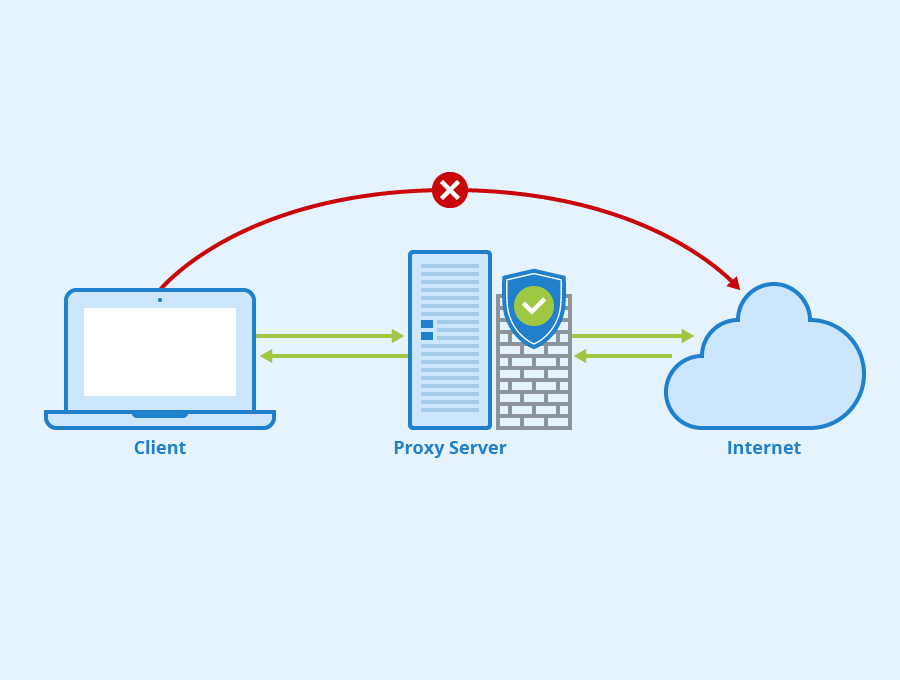
\includegraphics[width=10cm,trim={0 2cm 0 2cm},clip]{img/Proxy-Server}
	\caption{Communication to the Internet using a proxy server}
	\label{img:proxyServer}
\end{figure}

\pagebreak
The use of a web proxy also makes it easier for security operators to spot attempts to connect via HTTPS to the Internet without using the company's proxy, indicating bad configurations or unwanted software. These connections are usually rejected and logged into the security systems.

Moreover, credentials are frequently required to use a proxy, so an attacker needs to do a little research, either looking for the credentials on the computer or checking if it uses Active Directory tickets, in order to connect to external servers.

For all these reasons, it is very important to \underline{check for web proxy configurations} on the compromised system \underline{before attempting to do a web connection} to the Internet. As only HTTP/S protocols are affected by web proxies, other protocols (like DNS or ICMP) are safe to use instead.

\subsubsection{User and process permissions}
Another extremely useful information to obtain from the computer is related to privileges, as some techniques can only be deployed with elevated permissions. Consequently, it is important to: 
\begin{itemize}
\item Check if the user that is running the program has privileges: \textit{root} or \textit{sudoer} in Linux, \textit{Administrator} in Windows.
\item Check if the process is being run elevated (with privileges).
\end{itemize}

Permissions are not only useful in the compromised machine, but they can also make a difference if working within an Active Directory, as there are users that can launch privileged processes in multiple computers (depending on the role of the user).

When a machine is compromised, it is common to launch some techniques linked to the tactic "\textit{Privilege Escalation}" if the user compromised is not an \textit{Administrator}. And for this reason, there are also security mechanisms like Windows User Access Control (UAC), that ask the user if they are trying to run a program with privileges before actually running it.

\subsubsection{Common programs}
Finally, among the methods to deploy persistence, some involve using other software that has vulnerabilities or that can be hooked\footnotemark, to run malicious code when executed.
\footnotetext{ Hooking: techniques used to alter the behaviour of a program by intercepting function calls, messages, or events passed between software components}

This external software may even be something widely known or used, like the password manager \textit{Keepass}\cite{KeePassWeb} or the Subversion client \textit{TortoiseSVN}\cite{TortoiseSVNWeb}, that helps when doing code version controls. These two apps can be used when performing persistence on Windows with the tool \textit{SharPersist}\cite{SharPersist}, as explained in section \ref{sssec:windowsTools}.

%\footnotemark\footnotetext{ https://keepass.info/}
%\footnotemark\footnotetext{ https://tortoisesvn.net/}

\subsubsection{Domain or AD services}
Even though this project is not focused on domain (or Active Directory) persistence, it is worth mentioning that, when working in a machine inside a domain, it is very frequent to also study the domain characteristics and the role of the compromised user inside the domain.

There are different types of domain privileges, and while some allow applying persistence in the entire domain, others only affect a few computers. These privileges could prove useful, for example, when the compromised user has no privileges in the compromised machine, but using the default domain configuration, the adversary can hop to other machines, ending up in one where the user does have privileges. And privileges inside the domain are required in most domain persistence techniques.

Another interesting domain service is DNS servers, as they are essential to communicate machines inside a domain. Multiple techniques can be used to try to compromise DNS to get information (among other things), but, most importantly, certain techniques like "backdoors communication" sometimes do not work when using Internet DNS servers to resolve the adversary hostname, but they do work using internal DNS servers, so it is imperative to have them listed.
